
%(BEGIN_QUESTION)
% Copyright 2006, Tony R. Kuphaldt, released under the Creative Commons Attribution License (v 1.0)
% This means you may do almost anything with this work of mine, so long as you give me proper credit

A pine ``2 $\times$ 6'' board (actually 1.5 inches thick and 5.5 inches wide), 10 feet long, floats in water.  Its density is 26 lb/ft$^{3}$.  How far will it sink into the water while floating?  Hint: the board will float so that its ``6 inch'' dimension is parallel to the water's surface:

$$\includegraphics[width=15.5cm]{i00270x01.eps}$$

Hint: try the following ``thought experiments'' first.  Imagine a completely weightless board (wood density = 0.0 lb/ft$^{3}$) and determine the depth of submersion into the water.  Then, imagine a board whose density is exactly equal to that of water (wood density = 62.428 lb/ft$^{3}$) and determine the depth of submersion.  Finally, imagine a board with a density exactly equal to half that of water (31.214 lb/ft$^{3}$) and determine its depth of submersion.  Do you see a pattern?

\vskip 10pt

Next, write an equation describing the percentage of submersion for an object given its density ($D_{o}$) and the density of the liquid ($D_{l}$).

\vfil 

\underbar{file i00270}
\eject
%(END_QUESTION)





%(BEGIN_ANSWER)

This is a graded question -- no answers or hints given!

%(END_ANSWER)





%(BEGIN_NOTES)

If the wood is weightless, it won't sink at all into the water but rather will float completely on the top.  Thus, its ``sink ratio'' will be zero.

\vskip 10pt

If the wood is equally dense as the water, it will sink completely into the water.  Thus, its ``sink ratio'' will be 100\%.

\vskip 10pt

If the wood is half as dense as the water, it will sink half-way into the water.  Thus, its ``sink ratio'' will be 50\%.

\vskip 10pt

The pattern in these thought experiments should be clear: the ratio of wood density to water density (i.e. its specific gravity) defines its sink ratio.

\vskip 10pt

Given that pine has a density of 26 lb/ft$^{3}$ and water has a density of 62.4 lb/ft$^{3}$, the sink ratio should be 41.67\%.  For a board that is 1.5 inches thick, this means it will sink 0.625 inches into the water.

\vskip 20pt

$$x = {D_o \over D_l}$$

\noindent
Where,

$x$ = sink ratio (0 = completely floating; 1 = completely submerged)

$D_o$ = density of object

$D_l$ = density of liquid

%INDEX% Physics, static fluids: buoyancy

%(END_NOTES)


